\documentclass[tikz,border=1mm]{standalone}
\usetikzlibrary{matrix,chains,positioning,decorations.pathreplacing,arrows,shapes.geometric}

% Code modified from here https://tex.stackexchange.com/questions/505741/architecture-neural-network-with-weights

\begin{document}
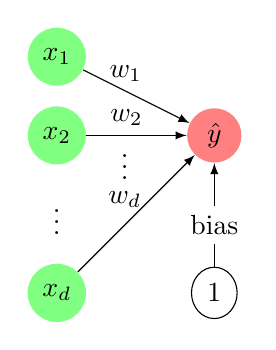
\begin{tikzpicture}[>=latex]
\path
(0,0)  node[circle,fill=green!50]  (x1) {$x_1$}
+(90:-1)    node[circle,fill=green!50]  (x2) {$x_2$}
+(90:-2) node  ()  {$\vdots$}
+(90:-3) node[circle,fill=green!50]  (xd) {$x_d$}
+(2, -3) node[ellipse, draw] (b) {1}
+(2,-1) node[circle,fill=red!50]  (y) {$\hat{y}$};

% +(-15:3) node[circle,fill=red!50]  (y2) {$\hat{y}_2$};
\draw[->] (x1)--(y) node[pos=.4,above]{$w_1$};
\draw[->] (x2)--(y) node[pos=.4,above]{$w_2$}; 
\draw[->] (xd)--(y) node[pos=.4,above=1mm]{$w_d$} node[pos=.4,above=4.5mm]{$\vdots$};
\draw[->] (b)--(y) node[pos=.4,fill=white]{bias}; 
\end{tikzpicture}
\end{document}